% ===== FRAME 13: Tabla de Desempeño Comparativo (MANTENER) =====
\begin{frame}[fragile,shrink=10]
  \frametitle{Resultados: Desempeño Comparativo}
  
  \begin{block}{Mejor modelo: \texttt{todos\_R01\_L5}}
    Resolución $R = 0{,}1°$, $\textcolor{ColorVerdeOliva}{\lambda = 5}$, datos completos ($\sim$744 reg/est)
  \end{block}
  
  \scriptsize
  \begin{table}
    \centering
    \begin{tabular}{lcccccc}
      \hline
      Modelo & Loss & MSE$_{u_x}$ & MSE$_{u_y}$ & MSE$_p$ & $\mathcal{R}_{NS}$ \\
      \hline
      \textbf{\textcolor{ColorVerdeOliva}{todos\_R01\_L5}} & 0,9261 & 0,4633 & 0,4347 & 1,3688 & \textbf{\textcolor{ColorRojoVino}{0,01273}} \\
      300xest\_R01\_L5 & 1,1207 & 0,4689 & 0,4647 & 1,6220 & 0,03682 \\
      300xest\_R04\_L1 & 1,0575 & 0,5059 & 0,5085 & 1,5720 & 0,24141 \\
      300xest\_R01\_L1 & 1,1380 & 0,4806 & 0,4756 & 1,6477 & 0,20107 \\
      300xest\_R04\_L10 & 1,0859 & 0,5220 & 0,5224 & 1,6185 & 0,02242 \\
      300xest\_R01\_L10 & 1,1624 & 0,4919 & 0,4966 & 1,6906 & 0,02318 \\
      \hline
    \end{tabular}
  \end{table}
  
  \normalsize
  \begin{itemize}
    \item Error observacional promedio: \alert{0,7556} (mejor entre todos)
    \item Residual Navier-Stokes: \alert{0,01273} (máxima coherencia física)
  \end{itemize}
  
  \note[item]{Tiempo: 1,5 minutos}
\end{frame}

% ===== FRAME 14: Análisis de Convergencia (MANTENER) =====
\begin{frame}[fragile]
  \frametitle{Resultados: Análisis de Convergencia}
  
  \begin{block}{Ranking por error observacional promedio}
    \begin{enumerate}
      \small
      \item (1) todos\_R01\_L5: 0,7556 (coherencia física: 0,01273)
      \item (2) 300xest\_R01\_L5: 0,8187 (coherencia física: 0,03682)
      \item (3) 300xest\_R01\_L10: 0,8267 (coherencia física: 0,02318)
    \end{enumerate}
  \end{block}
  
  \begin{columns}[T]
    \column{0.5\textwidth}
    \centering
    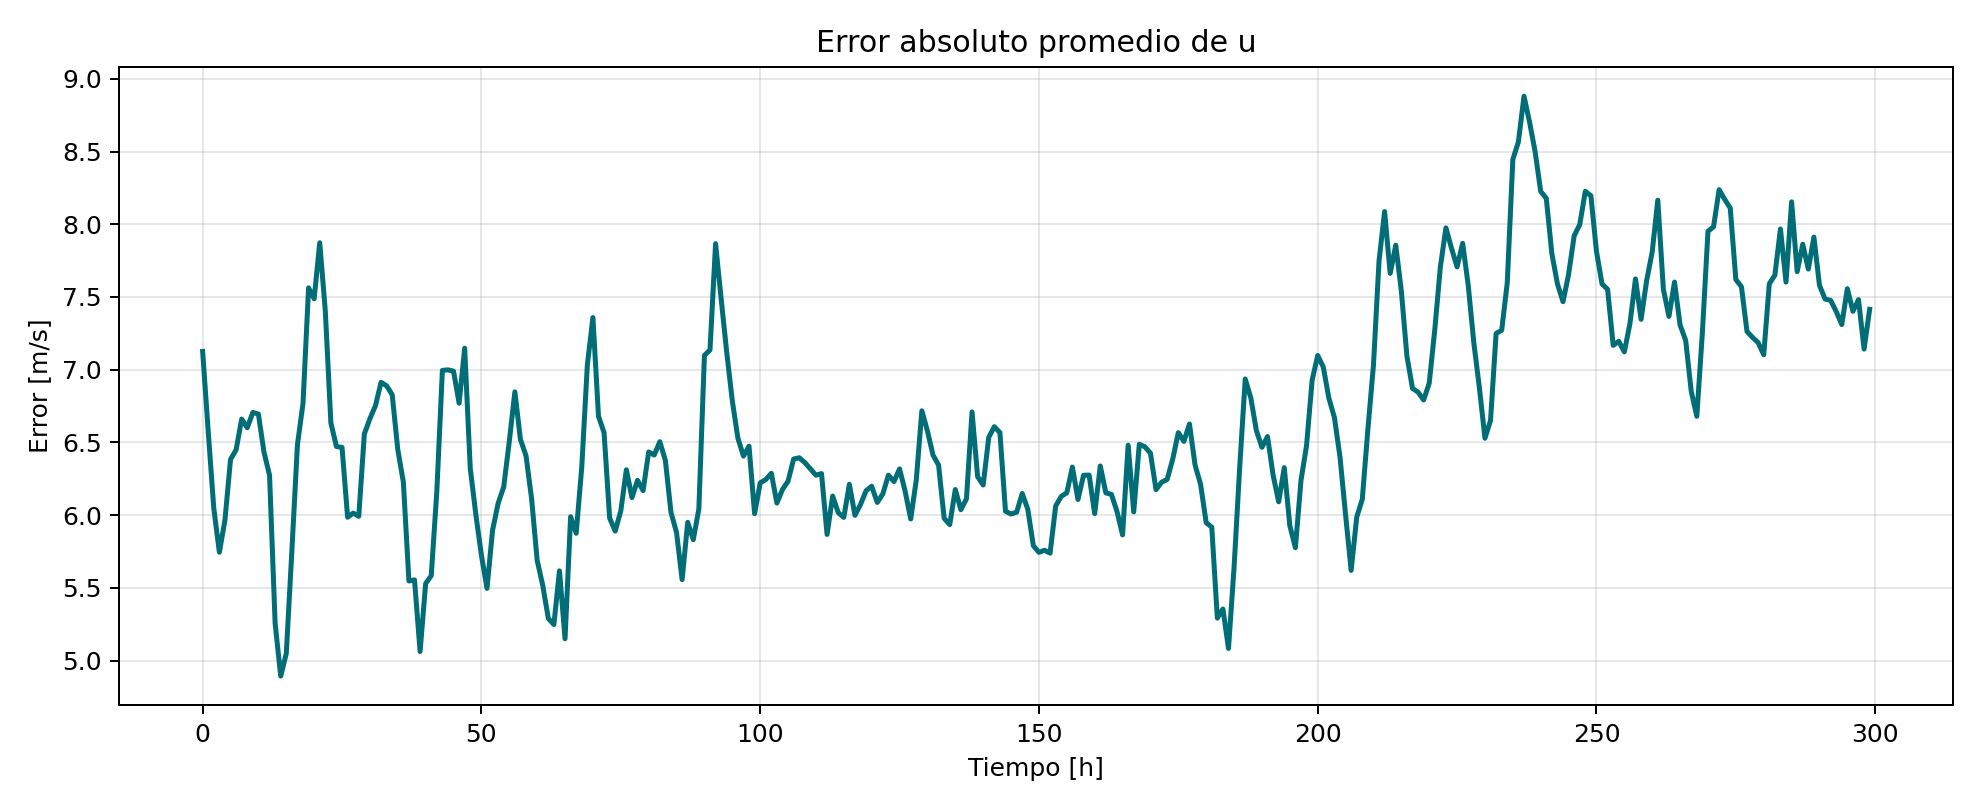
\includegraphics[width=\textwidth]{figures/error_u.png}
    \tiny Error promedio $u_x$ (m/s)
    
    \column{0.5\textwidth}
    \centering
    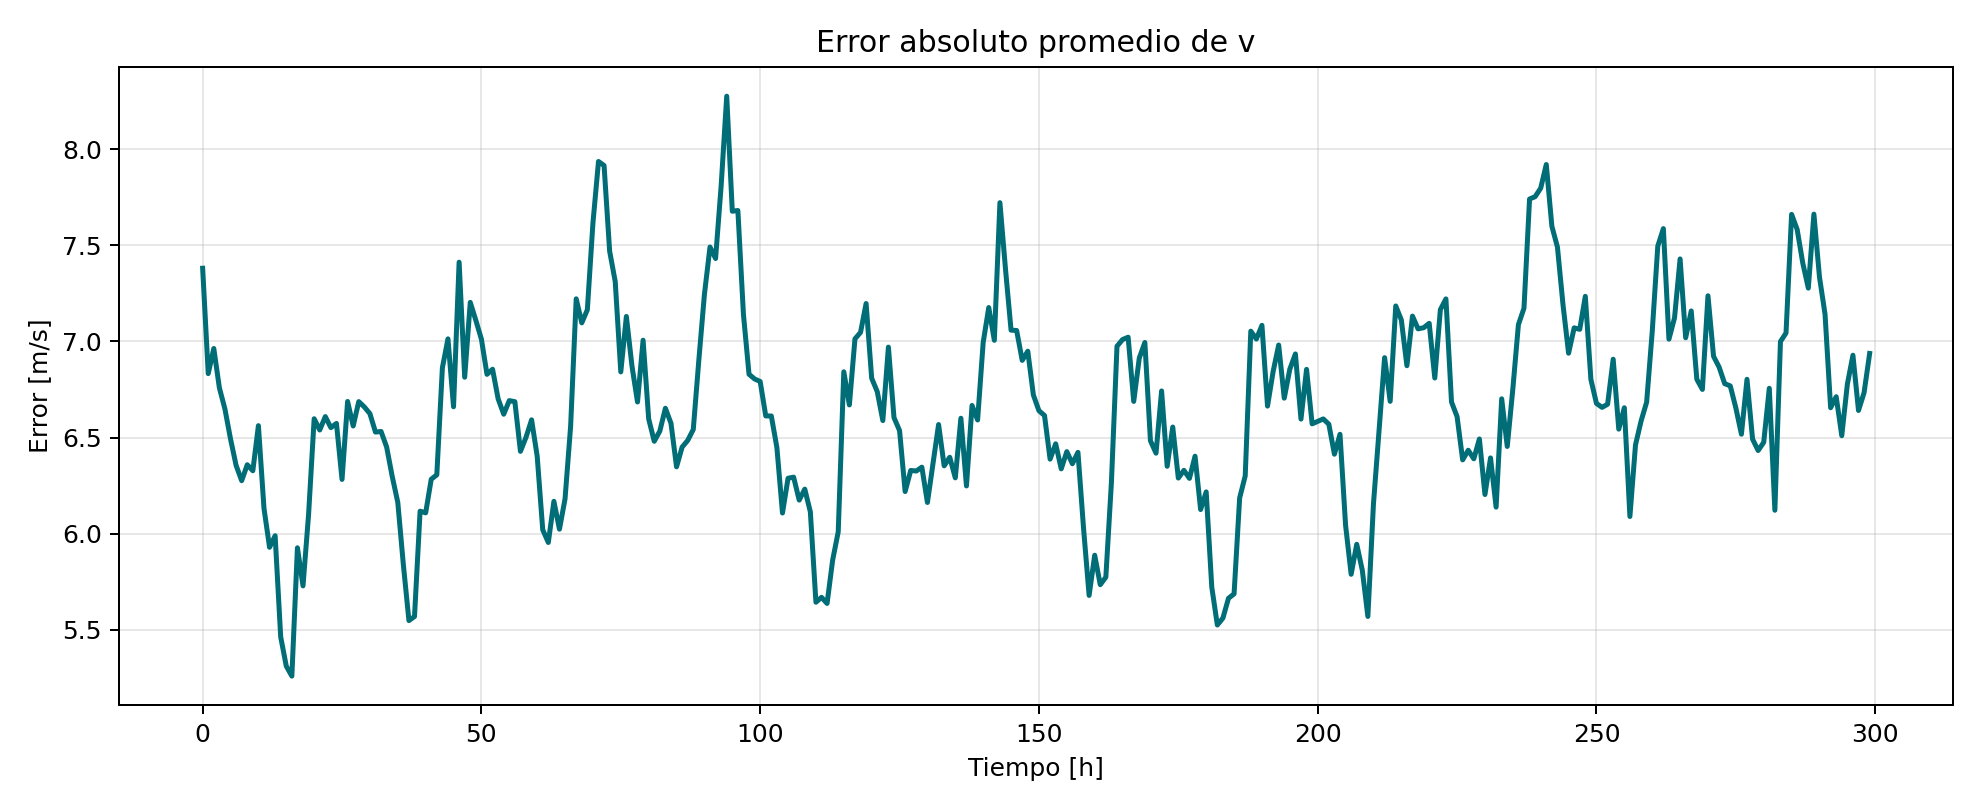
\includegraphics[width=\textwidth]{figures/error_v.png}
    \tiny Error promedio $u_y$ (m/s)
  \end{columns}
  
  \note[item]{Gráficos: Convergencia del error en componentes de viento}
  \note[item]{Tiempo: 1,5 minutos}
\end{frame}

% ===== FRAME 15: Validación Fuera de Muestra (NUEVA) =====
\begin{frame}[fragile,shrink=8]
  \frametitle{Resultados: Validación Fuera de Muestra}

  \begin{block}{Tabla 5.8: Comparación de métricas (train vs. test temporal)}
    \scriptsize
    \centering
    \begin{tabular}{lccc}
      \hline
      Métrica & Entrenamiento (días 1--20) & Prueba (días 21--31) & Diferencia \\
      \hline
      $\text{MSE}_{u_x}$ & 0{,}4633 & \textbf{0{,}4422} & $-4{,}5$\,\% \\
      $\text{MSE}_{u_y}$ & 0{,}4347 & \textbf{0{,}4248} & $-2{,}3$\,\% \\
      $\text{MSE}_{p}$   & 1{,}3688 & \textbf{3{,}9116} & $+185{,}8$\,\% \\
      $\mathcal{R}_{\text{NS}}$ & 0{,}01273 & \textbf{0{,}03640} & $+186{,}0$\,\% \\
      \hline
    \end{tabular}
  \end{block}

  \begin{block}{Lectura técnica}
    \begin{itemize}
      \small
      \item Generalización favorable en viento: $u_x$ y $u_y$ se mantienen estables en prueba.
      \item Brecha crítica en presión y residual físico: evidencia de dificultad de extrapolación temporal.
      \item Mensaje clave: buena robustez para velocidad, cautela para presión fuera del período de entrenamiento.
    \end{itemize}
  \end{block}

  \note[item]{Tiempo: 1,5 minutos}
  \note[item]{Fuente: Tabla 5.8 de la sección 5.5 (validación fuera de muestra)}
\end{frame}

% ===== FRAME 17: Análisis de Pérdida Total Comparativa (NUEVA) =====
\begin{frame}[fragile]
  \frametitle{Análisis: Comparativa de Pérdida Total}
  
  \begin{block}{Tabla 5.4: Comparación de resoluciones ($\overline{\text{MSE}}_{\text{obs}}$)}
    \scriptsize
    \centering
    \begin{tabular}{ccccc}
      \hline
      $\lambda$ & R=0,1 & R=0,4 & $\Delta$ (R0,4 - R0,1) & Mejor R \\
      \hline
      1  & 0,86796 & 0,86216 & -0,0058 & 0,4 \\
      3  & 1,24982 & 1,02208 & -0,2277 & 0,4 \\
      5  & 0,85185 & 1,32126 & +0,4694 & \textbf{0,1} \\
      10 & 0,89305 & 0,88765 & -0,0054 & 0,4 \\
      \hline
    \end{tabular}
  \end{block}

  \begin{block}{Lectura técnica}
    \begin{itemize}
      \small
      \item R=0,4 domina en $\lambda \in \{1,3,10\}$.
      \item El único caso donde la malla fina supera claramente es $\lambda = 5$.
      \item Decisión final: R=0,1 con $\lambda = 5$ por mejor equilibrio en el régimen óptimo.
    \end{itemize}
  \end{block}
  
  \note[item]{Tiempo: 1,5 minutos}
  \note[item]{Fuente: Tabla 5.4 (Comparación de resoluciones), doctg/18_resultados.tex}
\end{frame}

% ===== FRAME 18: Efecto de la Restricción Suave de Rango (NUEVA) =====
\begin{frame}[fragile]
  \frametitle{Resultados: Efecto de la Restricción Suave de Rango}

  \begin{block}{Tabla 5.6: Comparación de pérdida final (época 2.000)}
    \scriptsize
    \centering
    \begin{tabular}{lccc}
      \hline
      Experimento & Registros totales & Mecanismo de rango & Loss final \\
      \hline
      \texttt{300xest\_R01\_L5} & 5.400 & No & 1,117 \\
      \texttt{todos\_R01\_L5} & 13.392 & No & 0,926 \\
      \texttt{todosreg\_R01\_L5\_rangeL05} & 13.392 & Sí & \textbf{0,638} \\
      \hline
    \end{tabular}
  \end{block}

  \begin{block}{Lectura técnica (sección 5.4.6)}
    \begin{itemize}
      \small
      \item Manteniendo $R=0{,}1^\circ$ y $\lambda=5$, activar rango reduce la loss final de 0,926 a 0,638.
      \item Reducción relativa frente al modelo equivalente sin rango: \textbf{-31,1\%}.
      \item La restricción de rango regulariza la optimización y mejora la plausibilidad del campo previo a visualizar $u$ y $v$.
    \end{itemize}
  \end{block}

  \note[item]{Tiempo: 1,5 minutos}
  \note[item]{Transición: esta mejora en loss se evidencia espacialmente en los campos predichos de velocidad}
\end{frame}

% ===== FRAME 19: Campos Predichos de Velocidad (NUEVA) =====
\begin{frame}[fragile]
  \frametitle{Resultados: Campos Predichos de Velocidad}

  \begin{block}{Interpretación física de la mejor corrida con restricción de rango}
    La configuración \texttt{todosreg\_R01\_L5\_rangeL05} no solo reduce la pérdida total,
    sino que genera campos espaciales continuos y físicamente plausibles para las componentes
    horizontales del viento sobre el dominio Caribe.
  \end{block}

  \begin{columns}[T]
    \column{0.5\textwidth}
    \centering
    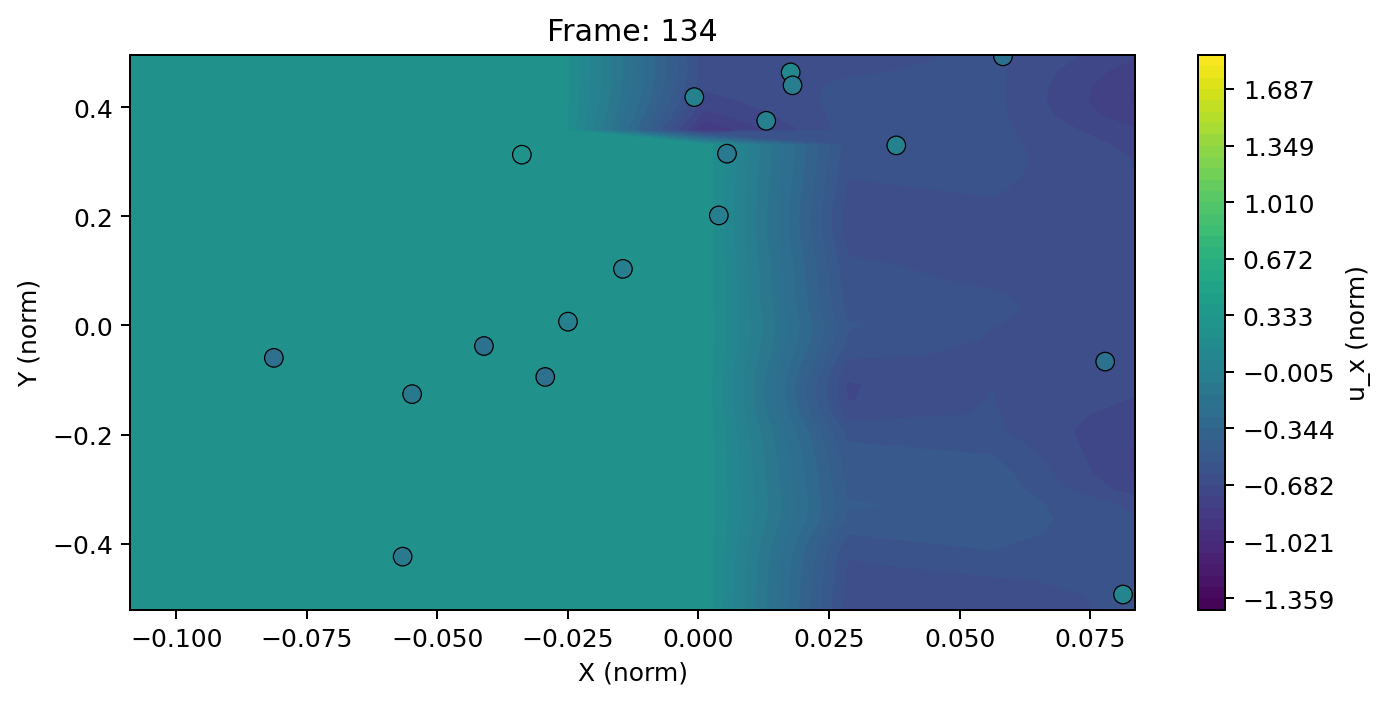
\includegraphics[width=\textwidth]{figures/pinn_campo_u_t134.png}
    \tiny Campo predicho final de $u$

    \column{0.5\textwidth}
    \centering
    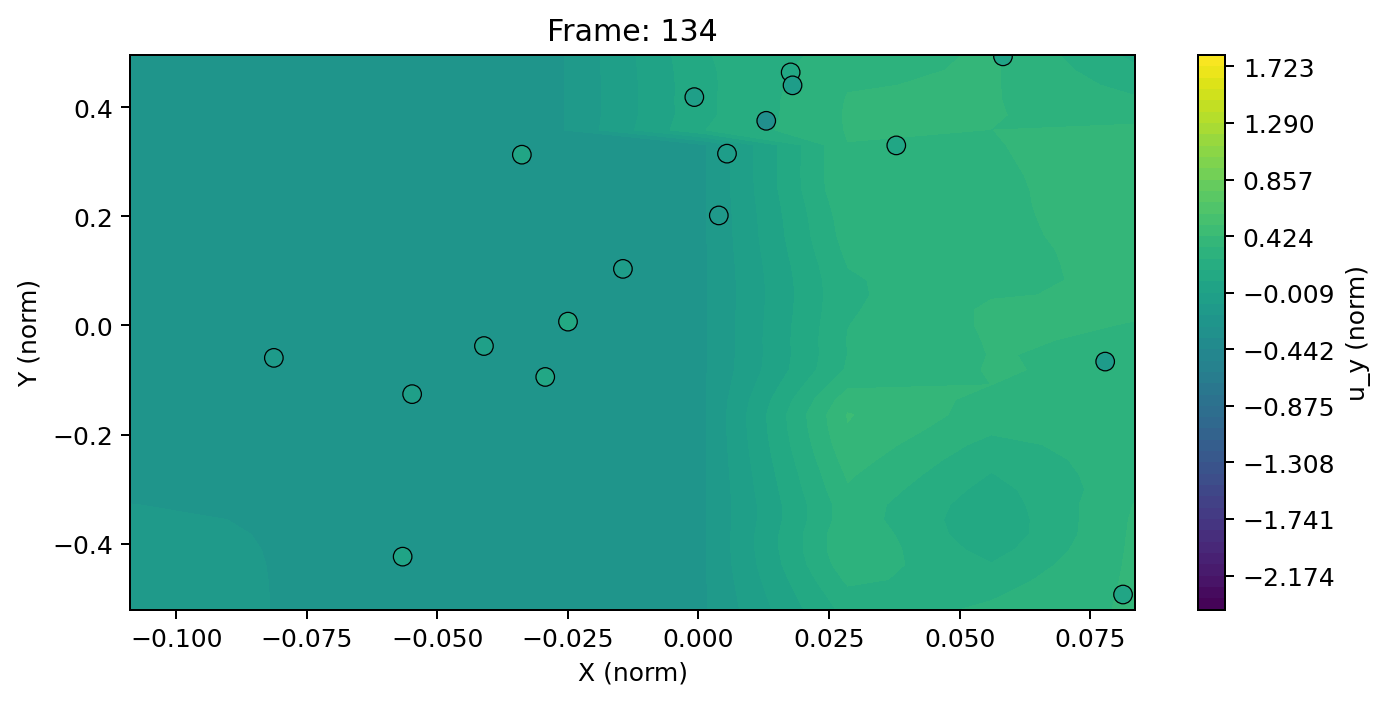
\includegraphics[width=\textwidth]{figures/pinn_campo_v_t134.png}
    \tiny Campo predicho final de $v$
  \end{columns}

  \note[item]{Tiempo: 1,5 minutos}
  \note[item]{Clave: traducir la mejora en pérdida a una evidencia espacial interpretable}
\end{frame}
